\documentclass[letterpaper]{article}
\usepackage[utf8]{inputenc}
\usepackage[spanish]{babel}
\usepackage{amssymb, amsmath}
\usepackage{stackengine}
\usepackage{graphicx}
\usepackage{lipsum}
\usepackage{dsfont}
\usepackage[margin=1.5cm,
vmargin={1.5cm,0.7cm},
includefoot]{geometry}
\usepackage{setspace}
\usepackage{subcaption}
\usepackage{tocloft}
\usepackage{upgreek}
\usepackage{amsthm}
\usepackage{graphicx}
\usepackage{paralist}
\usepackage{fancyhdr}
\usepackage{lmodern}
\usepackage{tcolorbox}
\usepackage{color}
\usepackage{tikz}
\usepackage{wasysym}
\usepackage{textgreek, marvosym}
\tcbuselibrary{skins,breakable}
\pagestyle{fancy}

\renewcommand{\headrulewidth}{0.4pt}
\renewcommand{\footrulewidth}{0.4pt}

\renewcommand{\d}{\partial}

\providecommand{\abs}[1]{\left|#1\right|}
\providecommand{\norm}[1]{\left|\left|#1\right|\right|}														  
\providecommand{\pint}[1]{\langle#1\rangle}														  
\newcommand{\V}{\mathds{V}}

\newcommand{\W}{\mathds{W}}

\newcommand{\F}{\mathds{F}}

\newcommand{\tq}{ \quad \cdot  \backepsilon \cdot \quad }

\newcommand{\ld}{\lim\limits_{x \to 0^{+}}}

\newcommand{\li}{\lim\limits_{x \to 0^{-}}}

\newcommand{\la}{\lim\limits_{x \to a}}

\renewcommand{\l}{\ell}

\newcommand{\R}{\mathds{R}}

\newcommand{\Po}{\mathds{P}_2(\mathds{R})}

\renewcommand{\*}{\cdot}

\newcommand{\Iden}{\begin{pmatrix}
		1 & 0 & 0\\
		0 & 1 & 0\\
		0 & 0 & 1 
\end{pmatrix}}
\newcommand{\T}{\begin{pmatrix}
		1 & 3 & 9 \\
		1 & 3 & 4 \\
		0 & 0 & 2 
\end{pmatrix} }

\makeatletter
\renewcommand*\env@matrix[1][\arraystretch]{%
	\edef\arraystretch{#1}%
	\hskip -\arraycolsep
	\let\@ifnextchar\new@ifnextchar
	\array{*\c@MaxMatrixCols c}}
\makeatother

\newtheorem{theorem}{Teorema}[]
\theoremstyle{definition}
\newtheorem{definition}{Definición}


\begin{document}
	
	\setlength{\unitlength}{1cm}
	\thispagestyle{empty}
	\begin{picture}(19,3)
	\put(-0.5,1.2){
\includegraphics[scale=.20]{img/unam1.png}}
	\put(16,1){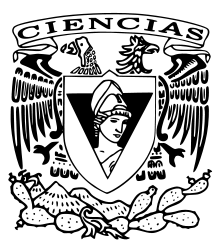
\includegraphics[scale=.29]{img/fciencias1.png}}
	\end{picture}
	
	\begin{center}
		\vspace{-114pt}
		\textbf{\large Matemáticas para las Ciencias II}\\
		\textbf{ Semestre 2020-2}\\
		Prof. Pedro Porras Flores\\
		Ayud. Irving Hernández Rosas \\
		\textbf{Proyecto V}\\[0.2cm]
		Kevin Ariel Merino Peña\footnote{Número de cuenta 317031326}\\ [0.2cm]
	\end{center}
	\vspace{-10pt}
	\rule{19cm}{0.3mm}
	
\noindent Realice los siguientes ejercicios, escribiendo el procedimiento claramente. Y recuerden que estos proyectos se entregan de manera individual en la plataforma de google classroom.\\


\noindent1.  Verifique el primer caso de la regla de la cadena de la composición $ f\circ \vec{\gamma}$ para cada uno de los siguientes casos, esto es primero haga la composición y derive, y le luego use la regla de la cadena y vea que se llega al mismo resultado.\\
\begin{theorem}[Regla de la cadena]
	\relax
	Sean $ U\subset \R^n $ y $ V \subset \R^m $ conjuntos abiertos, $ g: U \subset \R^n \to \R^m $ y $ f: V\subset \R^m \to \R^p $ dos funciones tales que $ g $ manda a $ U $ en $ V $ \textit{i.e. } $ f \circ g $. Supogamos que $ g $ es diferenciable en $ \vec{x_0} $ y $ D(f \circ g) (\vec{x_0}) = Df(g(\vec{x_0}))Dg(\vec{x_0}) $.\\
	\begin{itemize}
		\item \textbf{Primer caso de la regla de la cadena}\\
		
		Supongamos $ \vec{\gamma}: \R \to \R^3 $ es una trayectoria diferenciable y $ f: \R^3 \to \R $. Sea $ h(t) = f(\vec{\gamma})(t) = f(x(t), y(t), z(t)  $ donde 
		$ \vec{\gamma}(t)= (x(t),y(t),z(t)) $. Entonces
		\[  \dfrac{dh}{dt} = \dfrac{\d f}{\d x} \dfrac{dx}{dt} +  \dfrac{\d f}{\d y} \dfrac{dy}{dt} +  \dfrac{\d f}{\d z} \dfrac{dz}{dt} \]
		esto es:
		\[ \dfrac{dh}{dt} = \nabla f(\gamma(t)) \* \vec{\gamma'}(t) \] donde $ \vec{\gamma'}(t)= (x'(t),y'(t),z'(t))  $.
		
		\item  \textbf{Segundo caso de la regla de la cadena }\\
		
		Sean $ f:\R^3 \to \R $ y $ g:\R^3 \to \R^3 $. Escribimos 
		\[ g(x,y,z) = (u(x,y,x), v(x,y,z), w(x,y,z) \quad \text{  y  }\quad h(x,y,z) = f(u(x,y,z), u(x,y,z), w(x,y,z))  \]
		Entonces:
	\[ \begin{pmatrix}
	\dfrac{\d h}{\d x} & \dfrac{\d h}{\d y} & \dfrac{\d h}{\d x}
	\end{pmatrix} = \begin{pmatrix}
	\dfrac{\d f}{\d x} & \dfrac{\d f}{\d y} & \dfrac{\d f}{\d z}
	\end{pmatrix} \begin{pmatrix}[2]
	\dfrac{\d u}{\d x} & \dfrac{\d u}{\d x} & \dfrac{\d u}{\d x}\\
	\dfrac{\d v}{\d x} & \dfrac{\d v}{\d x} & \dfrac{\d v}{\d x}\\
	\dfrac{\d w}{\d x} & \dfrac{\d w}{\d x} & \dfrac{\d w}{\d x}\\
	\end{pmatrix} \]
	\end{itemize}
\end{theorem}

a) $f(x,y) = xy$, $\vec{\gamma}(t) =(e^t, \cos(t)) $.\\
Tenemos que $  f \circ \gamma(t) = e^t\cos(t) $ y su derivada es 
\begin{align*}
	\dfrac{d}{dt} (f\circ \gamma) &= \dfrac{d}{dt}e^t\cos(t) &&\text{Planteando la derivada}\\
	\dfrac{d}{dt} (f\circ \gamma) &= e^t\dfrac{d}{dt}\cos(t) + \cos(t)\dfrac{d}{dt}e^t &&\text{Por la regla del producto en derivadas}\\
	\dfrac{d}{dt} (f\circ \gamma) &= e^t(- \sin(t)) + \cos(t)e^t &&\text{Por nuestro curso de Cálculo I}\\
	\dfrac{d}{dt} (f\circ \gamma) &= e^t\cos(t) - e^t \sin(t) &&\text{Conmutando la suma de funciones}\\
\end{align*}
por otra parte, por el primer caso de la regla de la cadena, obtenemos
\[ 	\dfrac{d}{dt}(f\circ g) = 	\dfrac{df}{dx}\dfrac{dx}{dt} + \dfrac{df}{dy}\dfrac{dy}{dt} \]
entonces calculemos las siguientes derivadas
\begin{align*}
	\dfrac{\d f}{\d x}(xy) &= y &&\text{Por la regla del producto}\\
	\dfrac{\d f}{\d y}(xy) &= x &&\text{Por la regla del producto}\\
	\dfrac{dx}{dt}(e^t) &= e^t &&\text{Por propiedades de la exponencial}\\
	\dfrac{dy}{dt}(\cos(t)) &= -\sin(t) &&\text{Por características de las trigonométricas}\\
\end{align*}
Así, se tiene que 
\[ \dfrac{d}{dt}(f\circ g) = ye^t - x\sin(t) \] y como $ x = e^t $ y $ y = \cos(t) $
\[ \therefore  \qquad \dfrac{d}{dt}(f\circ g) = \cos(t)e^t-e^t\sin(t) \]


b) $f(x,y) = xy$, $\vec{\gamma}(t) =(3t^2, t^3) $.\\

Tenemos que $  f \circ \gamma(t) = e^{(3t^2)(t^3)} = e^{3t^5}  $ y su derivada es 

\begin{align*}
	\dfrac{d}{dt} (f\circ \gamma) &= \dfrac{d}{dt} e^{3t^5} &&\text{Planteando la derivada}\\
	\dfrac{d}{dt} (f\circ \gamma) &= e^{3t^5}\dfrac{d}{dt} 3t^5 &&\text{Por la regla de la derivada para la exponencial}\\
	\dfrac{d}{dt} (f\circ \gamma) &= e^{3t^5}(15t^4) &&\text{Derivando un monomio}\\
	\dfrac{d}{dt} (f\circ \gamma) &= 15t^4e^{3t^5} &&\text{Derivando un monomio}\\
\end{align*}
por otra parte, por el primer caso de la regla de la cadena, obtenemos
\[ 	\dfrac{d}{dt}(f\circ g) = 	\dfrac{df}{dx}\dfrac{dx}{dt} + \dfrac{df}{dy}\dfrac{dy}{dt} \]
entonces calculemos las siguientes derivadas
\begin{align*}
	\dfrac{\d f}{\d x}(e^{xy}) &= ye^{xy} &&\text{Por la regla de la exponencial}\\
	\dfrac{\d f}{\d y}(e^{xy}) &= xe^{xy} &&\text{Por la regla de la exponencial}\\
	\dfrac{dx}{dt}(3t^2) &= 6t &&\text{Por propiedades de la derivada en exponentes}\\
	\dfrac{dy}{dt}(t^3) &= 3t^2 &&\text{Por propiedades de la derivada en exponentes}\\
\end{align*}
Así, se tiene que 
\[ \dfrac{d}{dt}(f\circ g) = ye^{xy}(6t) - xe^{xy}(3t^2) \] y como $ x = 3t^2 $ y $ y = t^3 $
\[ \therefore  \qquad \dfrac{d}{dt}(f\circ g) = 15t^4e^{3t^5} \]

c) $f(x,y) = (x^2 + y^2)\ln{\sqrt{x^2 + y^2}}$, $\vec{\gamma}(t) =(e^t, e^{-t}) $.\\

Tenemos que $  f \circ \gamma(t) = (e^{2t} + e^{-2t})\ln \sqrt{e^{2t} + e^{-2t}}  $ y su derivada es 

\begin{align*}
\dfrac{d}{dt} (f\circ \gamma) &= \dfrac{d}{dt}((e^{2t} + e^{-2t})\ln \sqrt{e^{2t} + e^{-2t}})  &&\text{Planteando la derivada }\\
\dfrac{d}{dt} (f\circ \gamma) &= \dfrac{d}{dt}((e^{2t} + e^{-2t}) \* \dfrac{1}{2} \ln (e^{2t} + e^{-2t}))  &&\text{Pues } \ln(a^c) = c\* \ln(a)\\
\dfrac{d}{dt} (f\circ \gamma) &= \dfrac{1}{2} \ln (e^{2t} + e^{-2t})\*\dfrac{d}{dt}(e^{2t} + e^{-2t}) +  (e^{2t} + e^{-2t})\*\dfrac{d}{dt}\left(\dfrac{1}{2} \ln (e^{2t} + e^{-2t})\right)  && \text{Por regla del producto en derivadas}\\
\dfrac{d}{dt} (f\circ \gamma) &= \dfrac{1}{2} \ln (e^{2t} + e^{-2t})\*2(e^{2t} - e^{-2t}) +  (e^{2t} + e^{-2t})\*\dfrac{d}{dt}\left(\dfrac{1}{2} \ln (e^{2t} + e^{-2t})\right)  && \text{Derivando la primera parte}\\
\dfrac{d}{dt} (f\circ \gamma) &= \dfrac{1}{2} \ln (e^{2t} + e^{-2t})\*2(e^{2t} - e^{-2t}) +  \dfrac{e^{2t} + e^{-2t} (2e^{2t}-2e^{-2t})}{2\sqrt{e^{2t}+e^{-2t}}\sqrt{e^{2t}+e^{-2t}}} && \text{Derivando la segunda parte}\\
\dfrac{d}{dt} (f\circ \gamma) &= (e^{2t} - e^{-2t})(2\ln\sqrt{e^{2t} + e^{-2t} } + 1) && \text{Factorizando } (e^{2t} - e^{-2t})\\
\end{align*}
por otra parte, por el primer caso de la regla de la cadena, obtenemos
\[ 	\dfrac{d}{dt}(f\circ g) = 	\dfrac{df}{dx}\dfrac{dx}{dt} + \dfrac{df}{dy}\dfrac{dy}{dt} \]
entonces calculemos las siguientes derivadas
\begin{align*}
\dfrac{\d f}{\d x}((x^2 + y^2)\ln{\sqrt{x^2 + y^2}} ) &= x(2\ln\sqrt{x^{2} + y^{2}} + 1)  &&\text{Haciendo la parcial con }x\\
\dfrac{\d f}{\d y}((x^2 + y^2)\ln{\sqrt{x^2 + y^2}}) &= y(2\ln\sqrt{x^2 + y^2} + 1)  &&\text{El caso anterior es homólogo con }y\\
\dfrac{dx}{dt}(e^t) &= e^t &&\text{Por propiedades de la exponencial}\\
\dfrac{dy}{dt}(-e^t) &= -e^{-t} &&\text{Por propiedades de la exponencial }\\
\end{align*}
Así, se tiene que 
\[ \dfrac{d}{dt}(f\circ g) = x(2\ln\sqrt{x^{2} + y^{2}} + 1)\*e^t + y(2\ln\sqrt{x^2 + y^2} + 1)\*(-e^{-t}) \] y como $ x = e^t  $ y $ y = e^{-t} $
\[ \therefore  \qquad \dfrac{d}{dt}(f\circ g) = (e^{2t} - e^{-2t})(2\ln\sqrt{e^{2t} + e^{-2t} } + 1)  \]

d) $f(x,y) = xe^{x^2 + y^2}$, $\vec{\gamma}(t) =(t, -t) $.\\

Tenemos que $  f \circ \gamma(t) = te^{2t^2}   $ y su derivada es 

\begin{align*}
\dfrac{d}{dt} (f\circ \gamma) &= \dfrac{d}{dt} te^{2t^2} &&\text{Planteando la derivada }\\
\dfrac{d}{dt} (f\circ \gamma) &= t\dfrac{d}{dt} e^{2t^2}+e^{2t^2}\*\dfrac{d}{dt} t &&\text{Por propiedades de la multiplicación }\\
\dfrac{d}{dt} (f\circ \gamma) &= t\dfrac{d}{dt} e^{2t^2}+e^{2t^2}\*\dfrac{d}{dt} t &&\text{Por propiedades de la multiplicación }\\
\dfrac{d}{dt} (f\circ \gamma) &= t2e^{2t^2}\dfrac{d}{dt}t^2 + e^{2t^2} &&\text{La derivada de la exponencial es ella misma por la derivada de su argumento}\\
\dfrac{d}{dt} (f\circ \gamma) &= 4t^2e^{2t^2} + e^{2t^2} &&\text{Derivando un monomio}\\
\dfrac{d}{dt} (f\circ \gamma) &= e^{2t^2}(4t^2 + 1) &&\text{Empleando factor común}
\end{align*}
por otra parte, por el primer caso de la regla de la cadena, obtenemos
\[ 	\dfrac{d}{dt}(f\circ g) = 	\dfrac{df}{dx}\dfrac{dx}{dt} + \dfrac{df}{dy}\dfrac{dy}{dt} \]
entonces calculemos las siguientes derivadas
\begin{align*}
\dfrac{\d f}{\d x}(xe^{x^2+y^2} ) &= e^{x^2+y^2}(1+2x^2)  &&\text{Aplicando la parcial a la función }\\
\dfrac{\d f}{\d y}(xe^{x^2+y^2}) &= 2xye^{x^2+y^2} &&\text{Aplicando la parcial a la función }\\
\dfrac{dx}{dt}(t) &= 1 &&\text{Derivando un termino lineal}\\
\dfrac{dy}{dt}(-t) &= -1 &&\text{Derivando un término lineal }\\
\end{align*}
Así, se tiene que 
\[ \dfrac{d}{dt}(f\circ g) = e^{x^2+y^2}(1+2x^2) -2xye^{x^2+y^2}  \] y como $ x = t  $ y $ y = -t $
\[ \therefore  \qquad \dfrac{d}{dt}(f\circ g) = e^{2t^2}(1+4t^2)  \]



\noindent2. Sea $f(u, v, w) = (e^{u -w}, \cos{(u + v)} + \sin{(u + v + w)})$ y $g(x,y) = (e^{x}, \cos{(y - x)}, e^{-y} )$. Calcule $ f\circ g$ y $\mathbf{D}(f\circ g)(0,0)$.\\

\noindent3.  Calcule la derivada direccional de las siguientes funciones en el punto y la dirección dada: \\


a) $f(x,y) = x + 2xy -3y^2$, $(x_0, y_0) = (1,2)$ y $\vec{v} = \frac{3}{5}\hat{e}_1 + \frac{4}{5}\hat{e}_2 $.\\

b) $f(x,y) = \ln{\sqrt{x^2 + y^2}}$, $(x_0, y_0) = (1,0)$ y $\vec{v} = \left( \frac{1}{\sqrt{5}} \right)(2\hat{e}_1 + \hat{e}_2 )$.\\

c) $f(x,y) = e^x\cos{(\pi y)}$, $(x_0, y_0) = (0,-1)$ y $\vec{v} = - \left( \frac{1}{\sqrt{5}} \right)\hat{e}_1 +  \left( \frac{2}{\sqrt{5}} \right)\hat{e}_2 $.\\

d) $f(x,y) = xy^2 + x^3y$, $(x_0, y_0) = (4,-2)$ y $\vec{v} =  \left( \frac{1}{\sqrt{10}} \right)\hat{e}_1 +  \left( \frac{3}{\sqrt{10}} \right)\hat{e}_2 $.\\


\noindent4. Encuentre un vector que sea normal a la curva $x^3 + xy + y^3 = 11$ en  $(1,2)$.\\

\noindent5.  El Capitán Ralphis se encuentra en problemas cerca del lado soleado de Mercurio. La temperatura del casco del barco cuando está en la ubicación $(x, y, z)$ estará dada por $T(x,y,z) = e^{-x^2 - 2y^2 - 3z^2}$, donde $x,y,z$ se miden en metros. Actualmente está en $(1,1,1)$.\\

a) ¿En qué direcciones debería proceder para disminuir la temperatura más rápidamente?\\

b) Si el barco viaja a $e^8$ metros por segundo, ¿qué tan rápido será la disminución de la temperatura si avanza en esa dirección?\\

c) Desafortunadamente, el metal del casco se romperá si se enfría a una velocidad superior a $\sqrt{14}e^2$ grados por segundo. Describa el conjunto de posibles direcciones en las que puede proceder a bajar la temperatura a no más de esa tasa.\\






\end{document}
